% status: 100
% chapter: REST

\title{REST Abstract File System Service}


\author{Swarnima Sowani}
\affiliation{%
  \institution{Indiana University}
  \streetaddress{Smith Research Center}
  \city{Bloomington} 
  \state{IN} 
  \postcode{47408}
}
\email{shsowani@iu.edu}

\author{Gregor von Laszewski}
\affiliation{%
  \institution{Indiana University}
  \streetaddress{Smith Research Center}
  \city{Bloomington} 
  \state{IN} 
  \postcode{47408}
  \country{USA}}
\email{laszewski@gmail.com}


% The default list of authors is too long for headers}
\renewcommand{\shortauthors}{G. v. Laszewski}


\begin{abstract}
  We developed a REST Abstract File System Service which is a web
  services that implements and abstracts the underlying storage
  services and provides a uniform web services APIs for users to do
  file operations like, retrieving, storing, removing files on storage
  services. The service is provided to support storage engines such as
  Amazon Simple Storage Service, google drive and virtual
  machines. This service can be used by big data application clients
  to perform file operations with consolidated data view.
\end{abstract}

\keywords{hid-sp18-420, File system, abstraction, Amazon S3, Google drive, 
virtual 
machine}


\maketitle


\section{Introduction}

File system operations are an integral part of the operating system as
well as cloud services. They are a quintessential part of any big data
applications that deals with storing, retrieving or reading the
files. Modern distributed applications are likely to have data stored at
different locations with different storage systems. Managing the data
at the different locations is a difficult task.

There are numerous storage providers who facilitate their customers to
store, read, write, retrieve files. However, integrating with each one
of them is a potential tedious tasks since, understanding and
implementing APIs for each service is a time consuming.

This motivates the development of our \emp{REST Abstract File System
  Service}. It provides a layer of abstraction over the underlying
file system so that the users or customers can integrate storage
services as file systems like Amazon S3~\cite{hid-sp18-420-amazon-S3},
Google Drive~\cite{hid-sp18-420-google-drive} and other such services
without even knowing their implementation details. Because of the
abstraction, backend services can easily be switched while the client
application uses the same API to access the various services.


\begin{figure}[!ht]
        \centering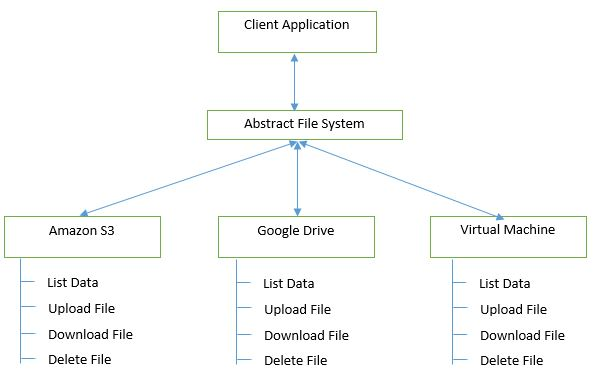
\includegraphics[width=\columnwidth]
        {image/architecture.JPG}
        \caption{System components}\label{fig:architecture}
\end{figure}


As shown in Figure~\ref{fig:architecture}, client applications can
interact with abstract file system with the web service package
provided. With the APis, it will be easy to perform file operations
such as listing, uploading, downloading and deleting in a uniform way
with supported storage engines.

With an abstract layer, all file operations will follow the same
process for all storage engines and it will be as easy as performing
operations on local system.


To get the clear understanding of application, Figure~\ref{fig:client}
shows a sample wireframe design of simple client application using
the REST Abstract File System Service.


\begin{figure}[!ht]
        \centering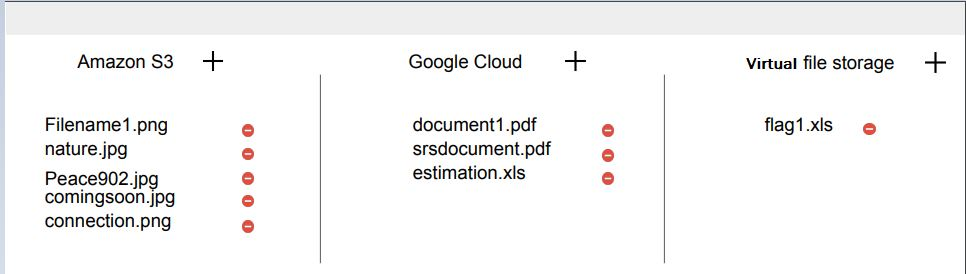
\includegraphics[width=\columnwidth]
        {image/client.JPG}
        \caption{Sample Client Application}\label{fig:client}
\end{figure}




\section{Technologies used}

The REST Abstract File System Service project is developed based on
different technologies. It is using Python as am implementation
language and APIs are generated using Swagger Codegen by reading
OpenAPI document.

\subsection{Python}

Python 2.7 is the underlying language that is used to implement all
the APIs provided by the REST Abstract File System Service.  There are
3 main python files having implementation of file operations to be
performed with Amazon S3, Google drive and Virtual machine storage
respectively. A number of python modules are used to support the
implemented functionality. Some of the important modules are

\begin{description}

\item[Boto3:] Boto3 is a software development kit (SDK) that provides
  AWS interface for Python applications. The REST Abstract File System
  Service is using Boto3 which is the latest version of the SDK
  provided. Boto 3 supports Python versions 2.6.5, 2.7 and 3.3
  version~\cite{hid-sp18-420-boto}.  It is used to support Amazon S3
  interface with the REST Abstract File System Service.

\item[ftplib:] The ftplib module in Python is used to perform
  different file opearations on virtual machine by connecting to FTP
  server installed on that machine~\cite{hid-sp18-420-FTP}.

\item[yaml:] This library is used to read the confog.yaml file used in
  the REST Abstract File System Service project to store the
  configurations required by different storage engines.

\item[google-api-python-client:] This is a python specific client
  library provided by google to handle the Google drive APIs.

\end{description}

These python modules are used in different python files to improve 
implemetation of abstract file system.

\subsection{Swagger}

Our \emph{REST Abstract File System Service} service is using Swagger Codegen
to generate server side stubs based on the abstractFileSystem.yaml
file with swagger specifications.  This yaml file is an OpenAPI
document which is in JSON format.  It contains swagger version, and
description of REST APIs.  Swagger was then used to install and run
REST service. It enabled APIs for accessing storage systems provided
in this project.

\section{Supported Storage Engines}

The REST Abstract File System Service Service developed by us, is currently
supporting three types of storage engines which are Amazon S3, Google
drive and any virtual machine. 

\subsection{Amazon S3}

Amazon S3 stands for Simple Storage Service. It is the most popular
storage service provided by Amazon Web
Service~\cite{hid-sp18-420-amazon-S3}. It provides a highly scalable,
reliable, and low latency data storage infrastructure at low
costs. Amazon S3 can be used to store and retrieve data of any kind
and any amount from anywhere. Amazon S3 is known for its durability
and stability. Amazon S3 SLAs claims to provide 99.999999999\%
durability for files stored in its durable
storage~\cite{hid-sp18-420-amazon-S3}. Amazon S3 is popularly an
object storage, where each file is treated as an object. Amazon S3
claims no cap on the amount of data that can be stored, that is why
companies who needs scale on the go prefer to choose Amazon S3 as
their file or object storage.

The REST Abstract File System Service encashes on the scalability and
simplicity Amazon S3 provides by abstracting the underlying mechanism
and providing a way to users to store their data into the durable S3
storage.

File operations supported by the REST Abstract File System Service
includes,

\begin{itemize}
\item Listing of files inside a specified bucket (bucket logical
  segregation of files)
\item Retrieving a specific file
\item Storing file in the specified bucket
\item Removing the file from the bucket
\end{itemize}



In order to use Amazon S3 as a storage system, first user needs to have an
account with AWS system.

To create new root account with AWS,
\begin{enumerate}
\item Go to AWS console and create new account.
\item Give details such as email address, password and user name.
\item Contact details: Give all specified contact details.
\item Payment Information: Give credit card or debit card details for
  user verification by AWS side.
\item Phone verification: AWS will make a call on the given number and
  give a 4 digit code to verify your phone number.
    \item Select a support plan and Continue.
\end{enumerate}



It is required to create new user in AWS account and give 
programmatic access so that the account credentials can be 
used for configuring with project.

\begin{enumerate}
    \item Login to AWS account.
    \item Go to Services and select IAM from drop down. 
	IAM stands for Access and Identity Management.
    \item Inside IAM resources, click on User.
    \item This will show the list of users. Click on Add User to add a new 
user.
    \item Provide user name and select programmatic access.
    \item On next page, provide optional permissions to user such as S3 Full
access and similar.
    \item On next page, review all settings and click Next.
    \item Access key and secret key are displayed here. Save it somewhere safe.
Key file can be downloaded here in \.csv format.
\end{enumerate}


To use Amazon S3 as a storage engine within Abstract File 
System, access key and secret key credentials must be provided in
the config.yaml file. The REST Abstract File System Service requires user to provide
four parameters to configure and start using Amazon S3 service.  (1)
Access Key, (2) Secret Key, (3) AWS region, and (4) Bucket name.


Access key and secret key are required for the programmatic
authentication of using S3 services. These keys are provided at the
time of user account creation with a role to access Amazon S3.  This
can be completed by following steps to create new user in AWS account
and give programmatic access section of this document.

Amazon S3 stores data within resources called bucket. Buckets are logical
segregation of files. Bucket name is configurable from the config.yaml file
which specifies the location where all file operations can be performed.

While creating a new bucket, an AWS region is assigned to that bucket. These 
buckets are globally unique and are accessible from anywhere. They are
placed in specific AWS region. AWS region is an area provided by AWS where
AWS resources available.

\subsection{Google Drive}

With 3 billion file uploads every day, Google drive is certainly one of the 
most popular and widely used storage provided by Google. Google drive offers 
its user a storage of 15 gigabytes for free and 100 gigabytes, 1 terabytes, 2 
terabytes, 10 terabytes, 20 terabytes and 30 terabytes through optional paid 
plans. Files uploaded in Google drive can be up to 5 terabytes in size. Google 
drive provides 99.9\% up-time guarantee~\cite{hid-sp18-420-google-drive-wiki}. 

Thw REST Abstract file system service provides integration with Google
drive so that they can use their existing account or new one to store
files seamlessly.

Abstract file system provides integration with Google drive by the means of 
API keys. 

File Operations Supported by the REST Abstract File System Service includes,
\begin{itemize}
    \item  Listing of files inside a drive
    \item  Retrieving a specific file 
    \item  Storing file inside drive
    \item  Removing the file from drive
\end{itemize}

Abstract file system requires user to login to their Google
account only for the first time of using this application and all
later requests will not require to authenticate again.

For the first request to Google drive API via Abstract file system, it
will open a browser for authentication. An existing account or new
account with Google is required for authentication.

User needs to perform authentication first and then Google drive will
ask user to allow or deny Abstract File system to access the Google
drive.

Figure~\ref{fig:auth} shows the screenshot of how authentication is 
required by application to access the Google drive data. 
The project registered with Google drive API has name file-system. 
Hence, Figure~\ref{fig:auth} shows that Google drive is asking user 
to allow or cancel file access to file-system application. 

\begin{figure}[!ht]
        \centering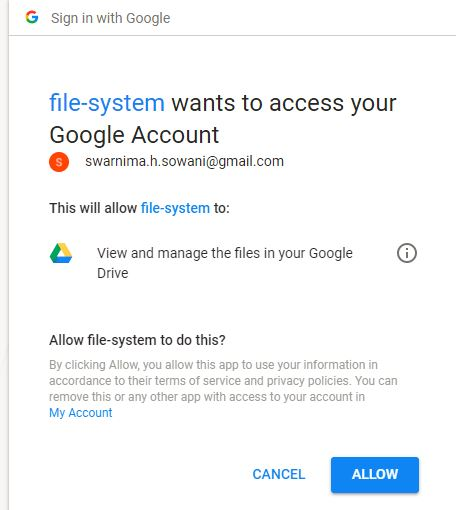
\includegraphics[width=\columnwidth]
        {image/auth.JPG}
        \caption{Aythentication for Google Drive}\label{fig:auth}
\end{figure}


Once user allows access to Abstract File system, user specific API
keys will be generated and stored inside google-drive-credentials.json
file.  For all later accesses of Abstract file system drive API, these
keys will be referred and there will be no need to login again.


\subsection{Virtual Machine}

The virtual machine on any cloud service provider can be used as a
storage. In certain scenarios, user needs to store the files on their
specific servers for variety of reasons. Abstract file system
facilitates storing the files on the server of their choice.

There can be multiple ways to access the storage provided by virtual
machines.

One way is to write an http service accept and transfer file and
storage on local file system and host this service on the virtual
machine. Second way could be to do SSH or SCP by writing a sub-process
for making a connection to machine using machines IP, port and
authentication through username, password or \verb|.pem| files. Third
way is to do FTP installation on virtual machine and using the newly
created FTP user in the program to access files on the virtual
machine.


The REST Abstract File System Service facilitates integration with any
virtual machine by the means of ftp installation. FTP is a file
transfer protocol and is a standard mechanism to deal with remote file
operations.


File Operations Supported by the REST Abstract File System Service include,
\begin{itemize}
    \item  Listing of files inside a specified folder allowed by ftp
    \item  Retrieving a specific file 
    \item  Storing file inside specified folder
    \item  Removing the file from the folder
\end{itemize}   

To use storage of some virtual machine, it is important to perform 
FTP installation on that server. 

Steps to install ftp on server~\cite{hid-sp18-420-FTP}
(Ubuntu Linux distribution is taken as example)


\begin{verbatim}
$ sudo apt-get install vsftpd
\end{verbatim}
%$

Edit the configuration file to allow writes to file system as well as
set the default file system path for file operations as
\verb|/srv/ftp|

\begin{verbatim}
$ sudo service vsftpd restart
\end{verbatim}
%$



Now make the ftp directory \verb|/srv/ftp| writable 


It is required to create a local file system user on the Virtual
Machine, you can do that by using following command

\begin{verbatim}
local_root = /srv/ftp  

write_enable=YES       

$ sudo adduser your_user_name    
\end{verbatim}
%$

This will ask for password and other details and will create a local
user on the virtual machine which can access the ftp installations.

Now everything is ready and abstract file system can make connection
with the file system of virtual machine.





Use \verb|config.yaml| file in for REST Abstract File System Service
to add the required details of Virtual machine.  It will be required
to provide details in config.yaml files to fill out hostname, port,
username, and password.


Host name is an IP address of the virtual machine which hosts the ftp 
installation. Port number is used to connect to the FTP on given port. By 
default port 21 is used for connection, and finally username and password of 
the FTP user created in FTP installation.





\section{Main Project Artifacts}

Thge REST Abstract File System Service uses different files. 
Each one of them is used for some specific function in this project.

\begin{description}



\item[abstractFileSystem.yaml:] This file is used for giving swagger
  specification for all the APIs used in the REST Abstract File System
  Service. This file will be used by Swagger code generator to create
  python stubs as per specification given in the yaml file.  This file
  contains swagger version, description, base path, path for each APIs
  respective input and output parameters of each API respectively.

\item[config.yaml:] This file is used to store the configurations
  required in the project.  Config.yaml file is used to store access
  key, secret key, bucket name and region for integrating Amazon S3 in
  the system. It also stores host name, port, username and password
  required to integrate virtual machine as a storage engine in the
  REST Abstract File System Service project.

\item[client\_id.json:] This file is used by Abstract File system to
  enable using google drive api in the project. This file is generated
  at the time of registering Abstract File System for API of Google
  drive. It has the key information that enables usage of google drive
  in this application.

\item[google\-drive\-credentials.json:] This file will store the keys
  of client who will be using Abstract File System. When any drive API
  is called for first time, it is required to login to the google
  drive and allow the REST Abstract File System Service to access the
  user drive.  After approval, user specific keys will be stored in
  google-drive-credentials.json file

\item[MakeFile:] MakeFile has different targets and it is used to
  build the project.  Make service is used for performing all the
  configurations required for the REST Abstract File System Service
  and then using swagger-codegen to generate code using swagger
  specification file abstractFileSystem.yaml. It will then copy all
  python files to the controller and download the requirements. Make
  start is used to run the service. Make clean is used to clean all
  the changes done while configuring the project.


  MakeFile also supports docker implementation. Make container is used
  to call docker-build and docker-start target which will generate
  docker container and run project services in the new container. Make
  docker-clean is used to stop the service and remove the container.

\item[DockerFile:]


  DockerFile is used to generate a docker image for the REST Abstract
  File System Service so it can be run.  It has specifications required for
  generating Ubuntu instance along with installation of python, java,
  curl, git, wget and required files to generate an image with all
  required installations ready. It then uses git repository by cloning
  inside image and then running a project based on targets available
  in the make file.

\item[all\_drive\_operations\_controller.py:] This is a python file
  that contains the code to implement required file operations for
  using Google drive as a storage engine in the REST Abstract File
  System Service.

\item[all\_s3\_operations\_controller.py:] This is a python file that
  contains the code to implement required file operations for using
  Amazon S3 as a storage engine in the REST Abstract File System
  Service.

\item[all\_vm\_operations\_controller.py:]

This is a python file that contains the code to implement required file 
operations for using virtual machine as a storage engine in Abstract File 
System. 

\end{description}



\section{Implementation results}

When no configurations present in config.yaml file, no storage 
system will be accessible it will be displayed as message in 
API result.


Figure~\ref{fig:not-configured} shows an output generated when none of
the storage engines is configured within the REST Abstract File System
Service.


\begin{figure*}[!ht]
        \centering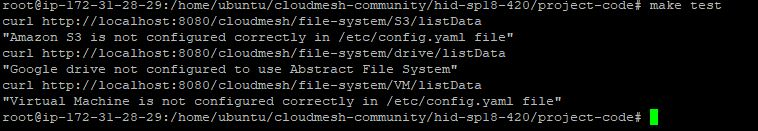
\includegraphics[width=\columnwidth]
        {image/not-configured.JPG}
        \caption{No storage system configured}\label{fig:not-configured}
\end{figure*}



All files listed from all storage engines,

APIs used:

\begin{itemize}
    \item /cloudmesh/file-system/S3/listData
    \item /cloudmesh/file-system/VM/listData
    \item /cloudmesh/file-system/drive/listData
\end{itemize}

Figure~\ref{fig:make-test} shows result of output by running make test 
command. Make test calls this listData API of all storage engines. 
Hence, it is displaying files from all 3 storage engines which are 
Amazon S3, Google Drive and Virtual Machine. 

\begin{figure*}[!ht]
        \centering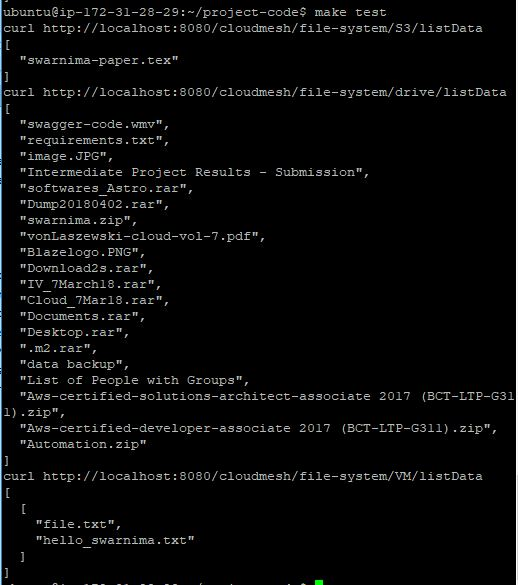
\includegraphics[width=\columnwidth]
        {image/make-test.JPG}
        \caption{all files from all engines}\label{fig:make-test}
\end{figure*}


To check file operations supported by the REST Abstract File System
Service to integrate with Amazon S3 these APIs are used,
\begin{itemize}
    \item /cloudmesh/file-system/S3/listData
    \item /cloudmesh/file-system/S3/downloadFile/{fileName}
    \item /cloudmesh/file-system/S3/uploadFile/{fileName}
    \item /cloudmesh/file-system/S3/deleteFile/{fileName}
\end{itemize}

Figure~\ref{fig:all-s3} shows all file operation performed by REST
Abstract File System Service with Amazon S3 as an underlying storage
engines.

\begin{figure*}[!ht]
        \centering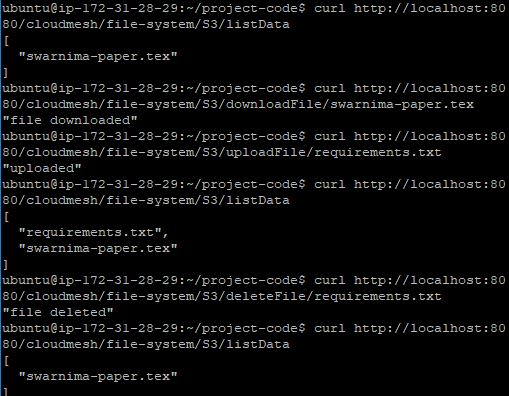
\includegraphics[width=\columnwidth]
        {image/all-s3.JPG}
        \caption{all S3 opearations}\label{fig:all-s3}
\end{figure*}


To check all file operations supported by the REST Abstract File
System Service to integrate with Virtual Machine storage these APIs
are used,

\begin{itemize}
    \item /cloudmesh/file-system/VM/listData
    \item /cloudmesh/file-system/VM/downloadFile/{fileName}
    \item /cloudmesh/file-system/VM/uploadFile/{fileName}
    \item /cloudmesh/file-system/VM/deleteFile/{fileName}
\end{itemize}

Figure~\ref{fig:VM} shows all file operation performed by Abstract 
File System with Virtual Machine as an underlying storage engines. 

\begin{figure*}[!ht]
        \centering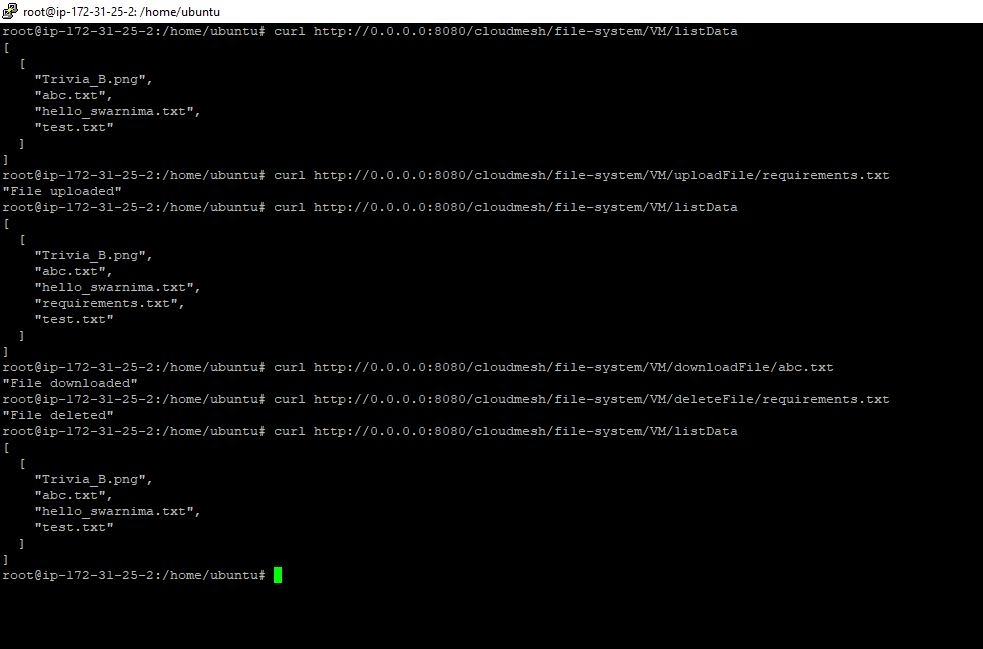
\includegraphics[width=\columnwidth]
        {image/VM.JPG}
        \caption{all VM opearations}\label{fig:VM}
\end{figure*}


To check all file operations supported by the REST Abstract File
System Service to integrate with Google Drive these APIs are used,

\begin{itemize}

    \item /cloudmesh/file-system/drive/listData
    \item /cloudmesh/file-system/drive/downloadFile/{fileName}
    \item /cloudmesh/file-system/drive/uploadFile/{fileName}
    \item /cloudmesh/file-system/drive/deleteFile/{fileName}

\end{itemize}

Figure~\ref{fig:drive-upload} shows output of file upload operation
performed by the REST Abstract File System Service with Google Drive
as an underlying storage engines.

\begin{figure*}[!ht]
        \centering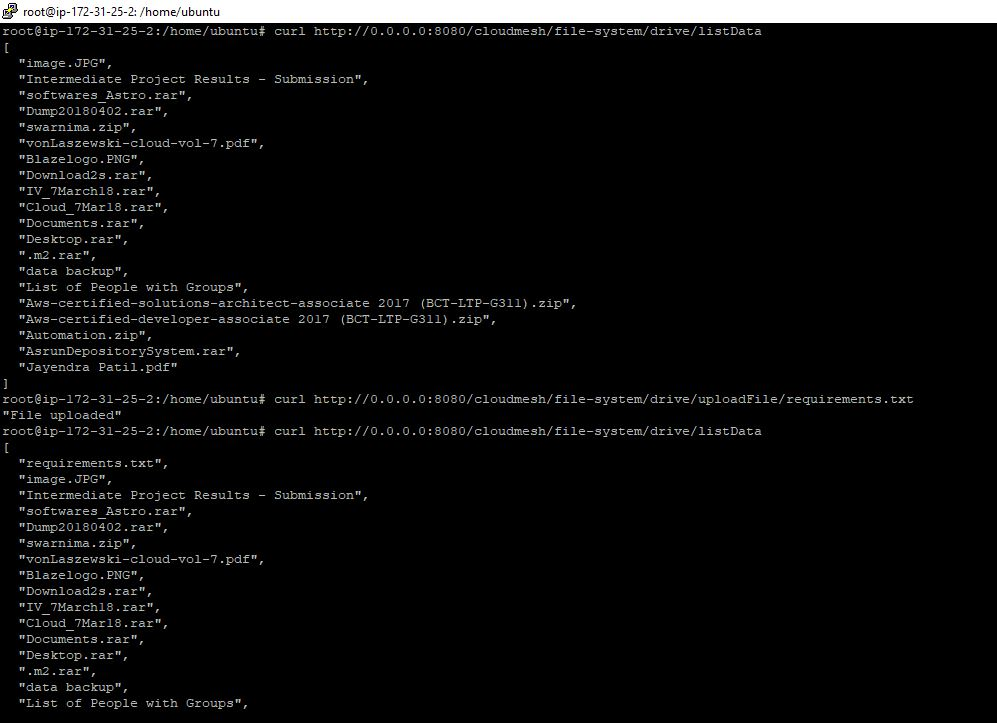
\includegraphics[width=\columnwidth]
        {image/drive-upload.JPG}
        \caption{Drive upload opearations}\label{fig:drive-upload}
\end{figure*}


Figure~\ref{fig:drive-delete} shows output of file delete operation
performed by the REST Abstract File System Service with Google Drive
as an underlying storage engines.

\begin{figure*}[!ht]
        \centering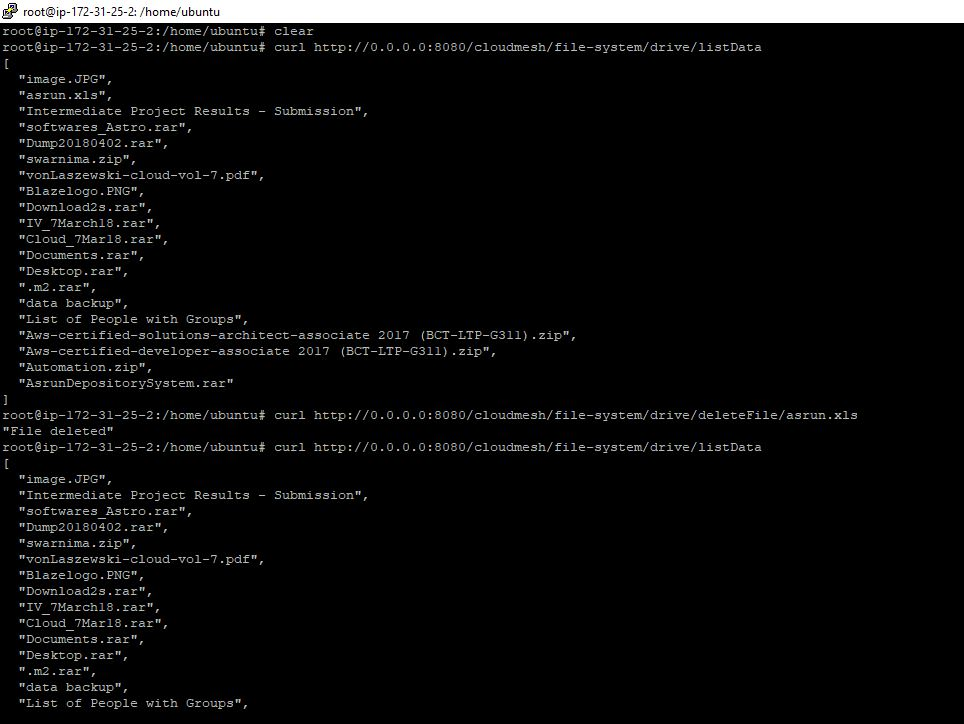
\includegraphics[width=\columnwidth]
        {image/drive-delete.JPG}
        \caption{Drive delete opearations}\label{fig:drive-delete}
\end{figure*}


Figure~\ref{fig:drive-download} shows output of file download
operation performed by the REST Abstract File System Service with
Google Drive as an underlying storage engines.

\begin{figure*}[!ht]
        \centering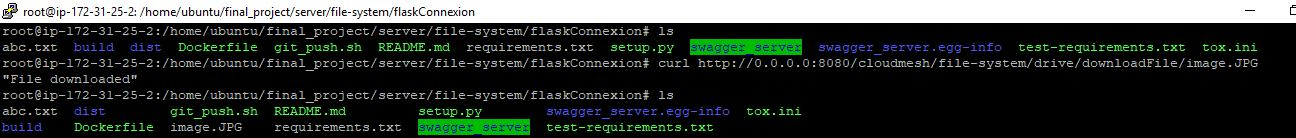
\includegraphics[width=\columnwidth]
        {image/drive-download.JPG}
        \caption{Drive download opearations}\label{fig:drive-download}
\end{figure*}


\section{Benefits of the REST Abstract File System Service}
\begin{enumerate}
    \item Since the REST Abstract File System Service abstracts the underlying storing 
mechanism, there is no need for client application to know 
the core implementation of the storage 
services like Amazon S3, Google Drive SDKs etc
    
    \item Switching between underlying storage mechanism is a hassle free task 
and can be done even by a newbie.
    
    \item Once abstract file system project is integrated into client 
applications, there is no code change required apart from only the 
configuration changes which are specific to underlying storage mechanism.
    
    \item Since the underlying storage mechanisms can be anything like Amazon 
S3, Google Drive which 
provides huge amount of data to be stored and retrieved on demand, scalability 
is the biggest benefit of abstract file system
	project
	
\item Abstract File system is currently dealing with only 3 types of
  storage engines which are Amazon S3, Google Drive and Virtual
  machines.  It is flexible to add other storage systems that can be
  configurable from config.yaml file and API specification provided in
  abstractFileSystem.yaml file.
    
\end{enumerate}


\section{Benchmarks}

Abstract File system project uses Amazon S3, google drive and Virtual
machine as its underlying storage engines. There are total 4 APIs
provided for each of the storage engine. The APis include listing of
files, file upload, download and deletion respectively.

In order to make use of this project, it is required to have access to
all these storage systems. To use Amazon S3, it is required to have an
account in AWS with a bucket created in S3 where file operations can
be performed. To use google drive as a storage system in this project,
user needs to have an account in google and it is required to login to
it when any of the Google drive API is called from the project for
first time. To use Virtual machine as a storage system, it is required
to complete FTP installation on the virtual machine and then the
credentials can be provided in the config.yaml file present in the
project to perform file operations on virtual machine.  In case if any
of the configuration is not available, abstract file system APIs call
to the respective storage engine will provide a response message
saying that this storage system is not configured.

The performance of all APIs is dependent upon the size of the file and
the speed of internet. System performance was tested with internet
speed of 4.29 mbps for upload and 6.1 mbps for download To test the
performance of list API to list files from each of the storage
engines, Amazon S3 took 0.01 seconds, Google drive took 0.02 seconds
and Virtual machine took 0.01 seconds.  To check the upload and
download APIs for each of the storage engines, a file with 87,856
kilobyte is used.

Figure~\ref{fig:upload-test} shows records of time taken 
by file upload operation on different storage systems

\begin{figure*}[!ht]
        \centering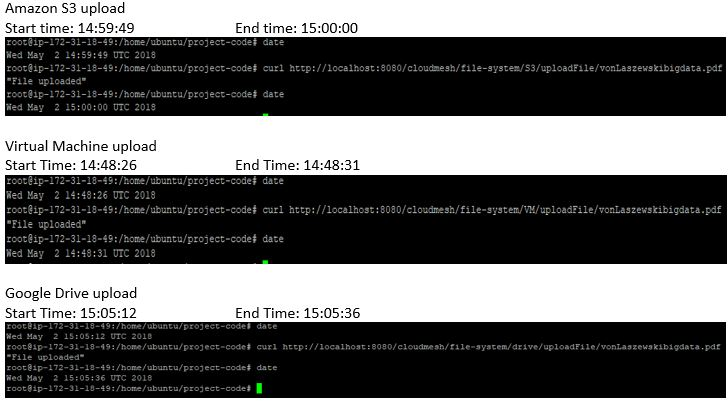
\includegraphics[width=\columnwidth]
        {image/upload-test.JPG}
        \caption{File upload performance test}\label{fig:upload-test}
\end{figure*}


Table~\ref{tab:timing} shows outcome of the performance test 
with number of seconds taken to execute all four APIs by different 
storage engines respectively.

\begin{table}[htb]
	\centering
  \caption{Processing time of all APIs for different storage 
  engines}\label{tab:timing}

	\begin{tabular}{*{4}{c}}
		\toprule
		APIs & Amazon S3 & Google Drive & Virtual Machine \\
		\midrule
		Listing & 0.01  & 0.02 & 0.01 \\
		Upload & 0.14 & 0.24 & 0.05 \\
        Download & 0.13 & 0.18 & 0.06 \\
        Delete & 0.04 & 0.06 & 0.02 \\
		\bottomrule
	\end{tabular}
\end{table}




\section{Challenges and Limitations}

The REST Abstract File System Service project requires a strong
internet connection.  Performance of the system is dependent on the
speed of internet.

The file name is passed as a URL parameter for APIs such as file upload,
file download. Abstract file system is not supporting multiple file 
upload and download at a time. Only one file can be uploaded or 
downloaded or deleted with one API call. 

No special security considerations are implemented other than those provided
by the underlaying subsystems.

\section{Conclusion}

The REST Abstract File System Service provides uniform APIs to perform
file operations on different storage systems in an abstract way. The
REST Abstract File System Service currently supports Amazon S3, Google
drive and Virtual machine as its storage engine. It can be scalable to
include other services as well.


Using the REST Abstract File system servuce allows to simplify the
tedious task to manage files between different storage providers. This
is achieved while using the same API by the client accessing different
storage engines in a seamless way.


By using the abstraction layer, storing or retrieving files from
different storage engines will be same process as being saved locally
or transferred over the network to other storage system. Such
abstraction makes it simpler to switch from one system to another
without having to rewrite vast swathes of application code.



\begin{acks}

  The author would like to thank Dr.~Gregor~von~Laszewski for his
  support and suggestions to write this paper.

\end{acks}

\bibliographystyle{ACM-Reference-Format}
\bibliography{report} 

